\chapter{Linear Models: Multiple variables and interactions}
\label{ch:MulExplInter}

Aims of this chapter\footnote{Here you work with the script file {\tt MulExplInter.R}}:
\begin{compactitem}
	\item Creating more complex models, including ANCOVA
	\item Looking at interactions between variables
	\item Plotting predictions from models
\end{compactitem}

We will look at two models in this chapter:
\begin{compactenum}
	\item Model 1: Is mammalian genome size predicted by interactions 
	between trophic level and whether species are ground dwelling?
	\item ANCOVA: Is body size in Odonata predicted by interactions 
	between genome size and taxonomic suborder?
\end{compactenum}

So far, we have only looked at the independent effects of variables. 
For example, in the trophic level and ground dwelling model from 
Chapter \ref{ch:MulExpl}, we only looked for specific differences for being a omnivore 
{\it or} being ground dwelling, not for being specifically a {\it 
ground dwelling omnivore}. These independent effects of a variable are 
known as {\it main effects} and the effects of combinations of 
variables acting together are known as {\it interactions} --- they 
describe how the variables {\it interact}.

\section{Formulae with interactions in R}

We've already seen a number of different model formulae in R. They all 
use this syntax:\\
 {\tt  response variable \textasciitilde\ explanatory variable(s)} \\
but we are now going to add two extra pieces of syntax:

\begin{compactdesc}
	\item [{\tt y \textasciitilde\  a + b + a:b}] The {\tt a:b} means the 
	interaction between {\tt a} and {\tt b} --- do combinations of these 
	variables lead to different outcomes?
	\item [{\tt y \textasciitilde\  a * b}] This a shorthand for the model 
	above. The {\tt *} means fit {\tt a} and {\tt b} as main effects and 
	their interaction {\tt a:b}.
\end{compactdesc}	 

\section{Model 1: Mammalian genome size}

\begin{compactitem}[$\quad\star$]
	\item Make sure you have changed the working directory to {\tt Code} 
	in your stats coursework directory.
	\item Create a new blank script called `Interactions.R' and add some 
	introductory comments.
	\item Use {\tt load('mammals.Rdata')} to load the data.
\end{compactitem}

If {\tt mammals.Rdata} is missing, just import the data again using 
{\tt read.csv("../Data/MammalData.csv")}. You will then have to add the 
log C Value column to the imported data frame again. 

Let's refit the model from Chapter \ref{ch:MulExpl}, but including the 
interaction between trophic level and ground dwelling. We'll 
immediately check the model is appropriate:

\begin{lstlisting}
> model <- lm(logCvalue ~ TrophicLevel * GroundDwelling, data= mammals)
> par(mfrow=c(2,2), mar=c(3,3,1,1), mgp=c(2, 0.8,0))
> plot(model)	
\end{lstlisting}

This gives:
\begin{center}
	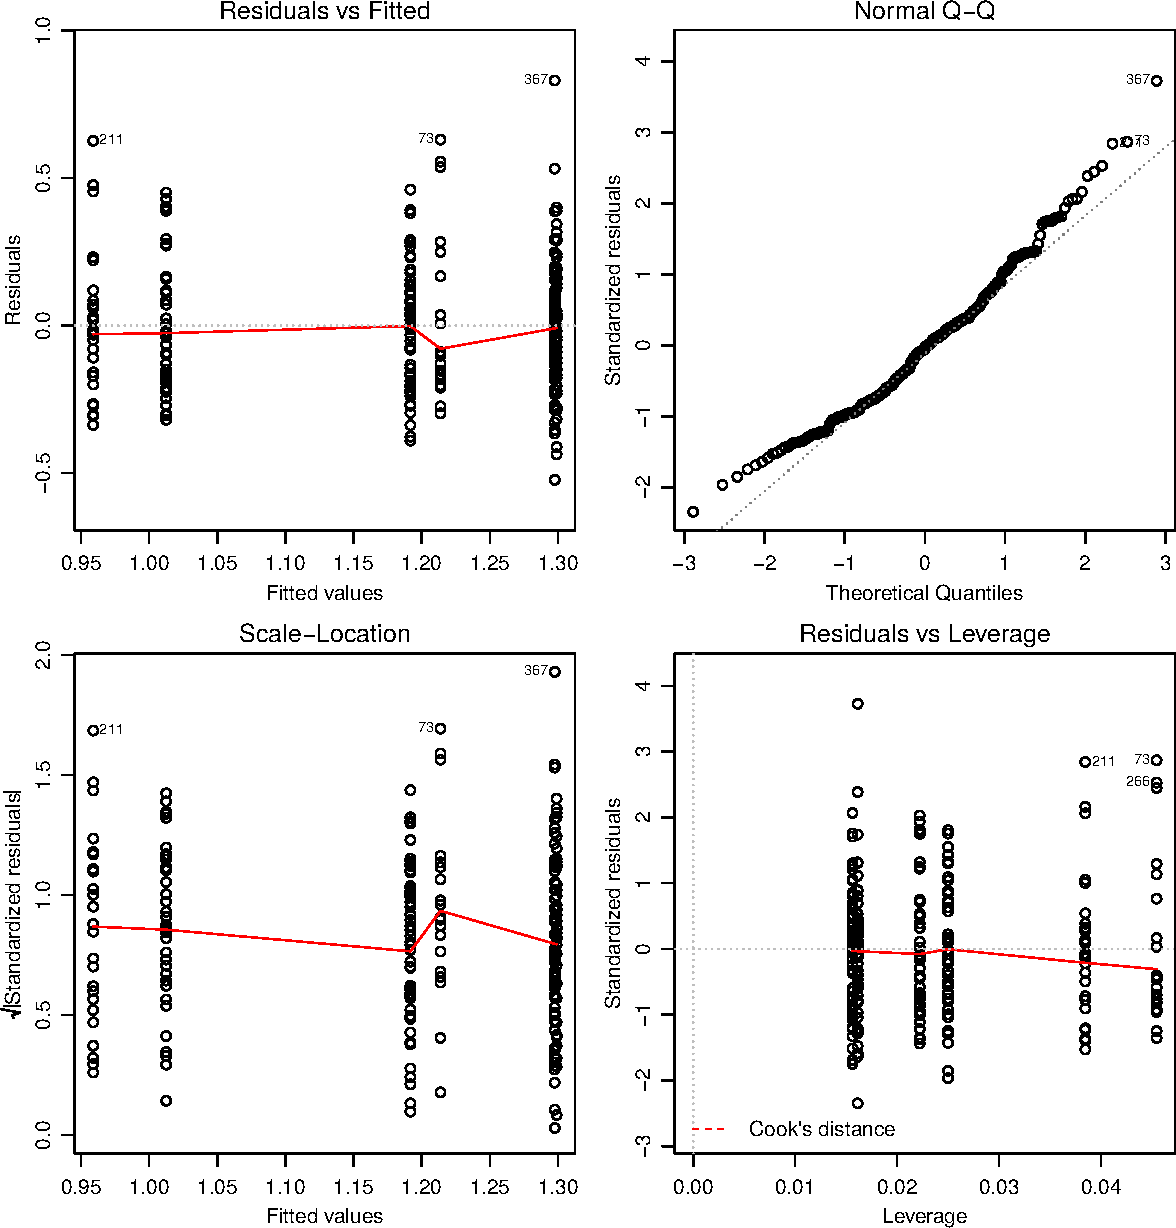
\includegraphics[width=\textwidth]{mamMod.pdf}
\end{center} 

Now, we'll examine the {\tt anova} and {\tt summary} outputs for the 
model:

\begin{lstlisting}
> anova(model)

 Analysis of Variance Table
 
 Response: logCvalue
                              Df Sum Sq Mean Sq F value  Pr(>F)    
 TrophicLevel                  2   0.81   0.407    8.06  0.0004 ***
 GroundDwelling                1   2.75   2.747   54.40 2.3e-12 ***
 TrophicLevel:GroundDwelling   2   0.43   0.216    4.27  0.0150 *  
 Residuals                   253  12.77   0.050                    
 ---
 Signif. codes:  0 '***' 0.001 '**' 0.01 '*' 0.05 '.' 0.1 ' ' 1 
\end{lstlisting}

Compared to the model from Chapter \ref{ch:MulExpl}, there is an extra line at the 
bottom. The top two are the same and show that trophic level and ground 
dwelling both have independent main effects. The extra line shows that 
there is also an interaction between the two. It doesn't explain a huge 
amount of variation, about half as much as trophic level, but it is 
significant.

Again, we can calculate the $r^2$ for the model: \[ \frac{0.81 + 2.75 + 
0.43}{0.81+2.75+0.43+12.77} = 0.238 \] The model from Chapter 
\ref{ch:MulExpl} without the interaction had an $r^2 = 0.212$ --- our 
new model explains 2.6\% more of the variation in the data.

The summary table is as follows:

 \begin{lstlisting}
>summary(model)
 
 Call:
 lm(formula = logCvalue ~ TrophicLevel * GroundDwelling, data = mammals)
 
 Residuals:
    Min     1Q Median     3Q    Max 
 -0.523 -0.171 -0.010  0.119  0.831 
 
 Coefficients:
                                         Estimate Std. Error t value Pr(>|t|)    
 (Intercept)                               0.9589     0.0441   21.76  < 2e-16 ***
 TrophicLevelHerbivore                     0.0535     0.0554    0.97  0.33460    
 TrophicLevelOmnivore                      0.2328     0.0523    4.45  1.3e-05 ***
 GroundDwellingYes                         0.2549     0.0651    3.92  0.00012 ***
 TrophicLevelHerbivore:GroundDwellingYes   0.0303     0.0786    0.39  0.69979    
 TrophicLevelOmnivore:GroundDwellingYes   -0.1476     0.0793   -1.86  0.06384 .  
 ---
 Signif. codes:  0 '***' 0.001 '**' 0.01 '*' 0.05 '.' 0.1 ' ' 1 
 
 Residual standard error: 0.225 on 253 degrees of freedom
   (120 observations deleted due to missingness)
 Multiple R-squared: 0.238,	Adjusted R-squared: 0.223 
 F-statistic: 15.8 on 5 and 253 DF,  p-value: 1.5e-13 
\end{lstlisting}

The lines in this are:
\begin{compactitem}
	\item The reference level (intercept) for non ground dwelling 
	carnivores. (The reference level is decided just by the alphabetic 
	order of the levels)
	\item Two differences for being in different trophic levels.
	\item One difference for being ground dwelling
	\item Two new differences that give specific differences for ground 
	dwelling herbivores and omnivores.
\end{compactitem}

The first four lines, as in the model from Chapter~\ref{ch:ANOVA}, 
which would allow us to find the predicted values for each group {\it if the size of the differences did not vary between levels because of the interactions}. That is, this part of the model only includes a single difference ground and non-ground species, which has to be the same for each trophic group because it  ignores interactions between trophic level and ground / non-ground
identity of each species. The last two lines then give the estimated coefficients associated with the interaction terms, and allow cause the size of differences to vary between levels because of the further effects of interactions.

The table below show how these combine to give the predictions for each 
group combination, with those two new lines show in red:

\[\begin{array}{|r|r|r|}
\hline
 & \textrm{Not ground} &  \textrm{Ground} \\
\hline
\textrm{Carnivore} & 0.96 = 0.96 &  0.96+0.25=1.21 \\
\textrm{Herbivore} & 0.96 + 0.05 = 1.01 & 0.96+0.05+0.25{\color{red}+0.03}=1.29\\
\textrm{Omnivore} & 0.96 + 0.23 = 1.19 & 0.96+0.23+0.25{\color{red}-0.15}=1.29\\
\hline
\end{array}\]

So why are there two new coefficients? For interactions between two 
factors, there are always $(n-1)\times(m-1)$ new coefficients, where 
$n$ and $m$ are the number of levels in the two factors (Ground dwelling or not: 2 levels and trophic level: 3 levels, in our current example). So in this model, $(3-1) \times (2-1) =2$. It is easier to understand why graphically: 
the prediction for the white boxes below can be found by adding the 
main effects together but for the grey boxes we need to find specific 
differences and so there are $(n-1)\times(m-1)$ interaction 
coefficients to add.

\[
n=4,m=4\quad
\begin{array}{|c|c|c|c|}
\hline
 & & & \\ 
\hline
 & \gc & \gc  &  \gc \\ 
\hline
 & \gc  & \gc  & \gc \\ 
\hline
 &  \gc &  \gc & \gc \\ 
\hline
\end{array}
\quad n=3,m=6 \quad
\begin{array}{|c|c|c|c|c|c|}
\hline
 & & & & &\\ 
\hline
 & \gc & \gc  &  \gc &  \gc &  \gc \\ 
\hline
 & \gc  & \gc  & \gc  &  \gc &  \gc\\ 
\hline
\end{array}
\]

If we put this together, what is the model telling us? 
\begin{compactitem}
\item Herbivores have the same genome sizes as carnivores, but 
omnivores have larger genomes.
\item Ground dwelling mammals have larger genomes.
\item These two findings suggest that ground dwelling omnivores should 
have extra big genomes. However, the interaction shows they are smaller 
than expected and are, in fact, similar to ground dwelling herbivores.
\end{compactitem}

Note that although the interaction term in the {\tt anova} output is 
significant, neither of the two coefficients in the {\tt summary} has a 
$p<0.05$. There are two weak differences (one very weak, one nearly 
significant) that together explain significant variance in the data.

\begin{compactitem}[$\quad\star$]
	\item Copy the code above into your script and run the model.
	\item Make sure you understand the output!
\end{compactitem}

Just to make sure the sums above are correct, we'll use the same code 
as in \ref{ch:MulExpl} to get R to calculate predictions for us: 

\begin{lstlisting}
# a data frame of combinations of variables
> gd <- rep(levels(mammals$GroundDwelling), times = 3)
> print(gd)
 [1] "No"  "Yes" "No"  "Yes" "No"  "Yes"

> tl <- rep(levels(mammals$TrophicLevel), each = 2)
> print(tl)

 [1] "Carnivore" "Carnivore" "Herbivore" "Herbivore" "Omnivore"  "Omnivore" 

# New data frame
> predVals <- data.frame(GroundDwelling = gd, TrophicLevel = tl)

# predict using the new data frame
> predVals$predict <- predict(model, newdata = predVals)
> print(predVals)
 
    GroundDwelling TrophicLevel predict
 1             No    Carnivore  0.9589
 2            Yes    Carnivore  1.2138
 3             No    Herbivore  1.0125
 4            Yes    Herbivore  1.2977
 5             No     Omnivore  1.1918
 6            Yes     Omnivore  1.2990
\end{lstlisting}

\begin{compactitem}[$\quad\star$]
	\item Run these predictions in your script.
\end{compactitem}

If we plot these data points onto the barplot from Chapter 
\label{ch:MulExpl}, they now lie exactly on the mean values, 
because we've allowed for interactions. The triangle on this plot shows 
the predictions for ground dwelling omnivores from the main effects 
($0.96 + 0.23  + 0.25 = 1.44$), the interaction of $-0.15$ pushes the 
prediction back down.

\begin{center}
	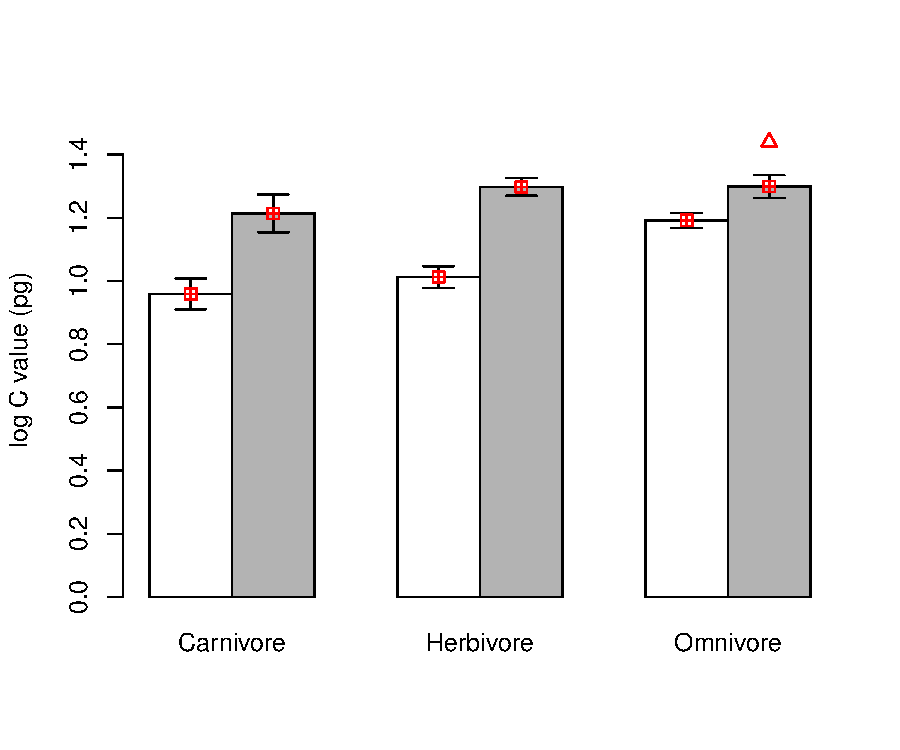
\includegraphics[width=0.8\textwidth]{predPlot.pdf} 
\end{center} 

\section{ANCOVA: Body Weight in Odonata}

We'll go all the way back to the regression analyses from 
Chapter~\ref{ch:regress}. Remember that we fitted two separate 
regression lines to the data for damselflies and dragonflies. We'll now 
use an interaction to fit these in a single model. This kind of linear 
model --- with a mixture of continuous variables and factors --- is 
often called an {\it analysis of covariance}, or ANCOVA. That is, 
ANCOVA is a type of linear model that blends ANOVA and regression. 
ANCOVA evaluates whether population means of a dependent variable are 
equal across levels of a categorical independent variable, while 
statistically controlling for the effects of other continuous variables 
that are not of primary interest, known as covariates. 

{\it That is, this is still a linear model, but with one categorical and one or more continuous predictors}.

\begin{compactitem}[$\quad\star$]
	\item Load the data: {\tt odonata <- read.csv('../Data/GenomeSize.csv')}.
	\item Create two new variables in the {\tt odonata} data set called 
	{\tt logGS} and {\tt logBW} containing log genome size and log body 
	weight.
\end{compactitem}

The models we fitted before looked like this:

\begin{center}
	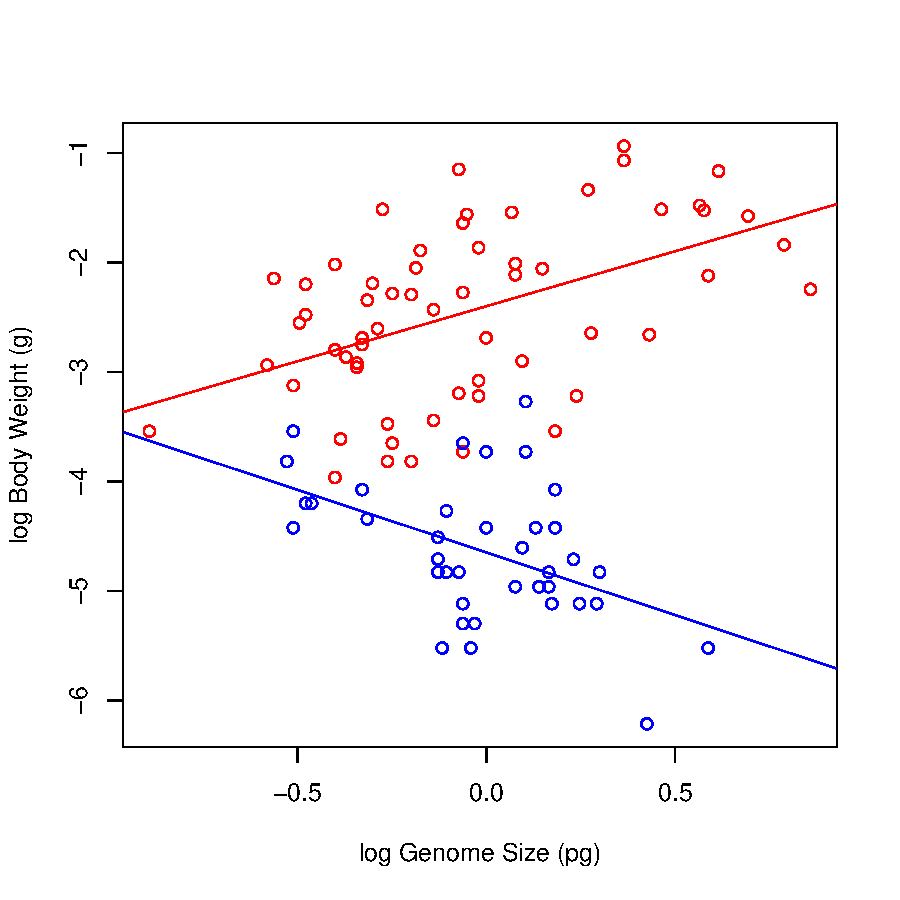
\includegraphics[width=0.7\textwidth]{dragonData.pdf} 
\end{center} 

We can now fit the model of body weight as a function of both genome 
size and suborder:

\begin{lstlisting}
> odonModel <- lm(logBW ~ logGS * Suborder, data = odonata)
\end{lstlisting}

Again, we'll look at the {\tt anova} table first:

\begin{lstlisting}
> anova(odonModel)
 
 Analysis of Variance Table
 
 Response: logBW
                Df Sum Sq Mean Sq F value  Pr(>F)    
 logGS           1    1.1     1.1    2.71     0.1    
 Suborder        1  112.0   112.0  265.13 < 2e-16 ***
 logGS:Suborder  1    9.1     9.1   21.65 1.1e-05 ***
 Residuals      94   39.7     0.4                    
 ---
 Signif. codes:  0 '***' 0.001 '**' 0.01 '*' 0.05 '.' 0.1 ' ' 1 
\end{lstlisting}

Interpreting this gives the following:
\begin{compactitem}

	\item There is no significant main effect of log genome size. The 
	{\it main} effect is the important thing here --- genome size is 
	hugely important but does very different things for the two different 
	suborders. If we ignored {\tt Suborder}, there isn't an overall 
	relationship: the average of those two lines is pretty much flat.

	\item There is a very strong main effect of Suborder: the mean body 
	weight in the two groups are very different.

	\item There is a strong interaction between suborder and genome size. 
	This is an interaction between a factor and a continuous variable and 
	shows that the {\it slopes} are different for the different factor 
	levels.

\end{compactitem}
	
The summary table looks like this:
\begin{lstlisting}
> summary(odonModel)
 
 Call:
 lm(formula = logBW ~ logGS * Suborder, data = odonata)
 
 Residuals:
     Min      1Q  Median      3Q     Max 
 -1.3243 -0.3225  0.0073  0.3962  1.4976 
 
 Coefficients:
                         Estimate Std. Error t value Pr(>|t|)    
 (Intercept)              -2.3995     0.0848  -28.31  < 2e-16 ***
 logGS                     1.0052     0.2237    4.49  2.0e-05 ***
 SuborderZygoptera        -2.2489     0.1354  -16.61  < 2e-16 ***
 logGS:SuborderZygoptera  -2.1492     0.4619   -4.65  1.1e-05 ***
 ---
 Signif. codes:  0 '***' 0.001 '**' 0.01 '*' 0.05 '.' 0.1 ' ' 1 
 
 Residual standard error: 0.65 on 94 degrees of freedom
   (2 observations deleted due to missingness)
 Multiple R-squared: 0.755,	Adjusted R-squared: 0.747 
 F-statistic: 96.5 on 3 and 94 DF,  p-value: <2e-16 
 
\end{lstlisting}

The first thing to note is that the $r^2$ value is really high. The 
model explains three quarters (0.752) of the variation in the data. 
Next, there are four coefficients:

\begin{compactitem}
	\item The intercept is for the first level of {\tt Suborder}, which 
	is Anisoptera (dragonflies).
	\item The next line, for log genome size, is the slope for Anisoptera.
	\item We then have a coefficient for  the second level of {\tt 
	Suborder}, which is Zygoptera (damselflies). As with the first model, 
	this difference in factor levels is a difference in mean values and 
	shows the difference in the intercept for Zygoptera. 
	\item The last line is the interaction between {\tt Suborder} and 
	{\tt logGS}. This shows how the slope for Zygoptera differs from the 
	slope for Anisoptera.
\end{compactitem}

How do these hang together to give the two lines shown in the model? We 
can calculate these by hand:
\begin{align*}
	\textrm{Body Weight} &= -2.40 + 1.01 \times \textrm{logGS} & \textrm{[Anisoptera]}\\
	\textrm{Body Weight} &= (-2.40 -2.25) + (1.01 - 2.15) \times \textrm{logGS} & \textrm{[Zygoptera]}\\
	                     &= -4.65 - 1.14 \times \textrm{logGS} \\
\end{align*}


\begin{compactitem}[$\quad\star$]
	\item Add the code into your script and check that you understand the 
	outputs.
\end{compactitem}

We'll use the {\tt predict} function to get the predicted values from 
the model and add lines to the plot above.

First, we'll create a set of numbers spanning the range of genome size:

\begin{lstlisting}	
#get the range of the data
> rng <- range(odonata$logGS)
#get a sequence from the min to the max with 100 equally spaced values
> LogGSForFitting <- seq(rng[1], rng[2], length = 100)
\end{lstlisting}
Have a look at these numbers:
 
\begin{lstlisting}	
	print(LogGSForFitting)
\end{lstlisting}
 
We can now use the model to predict the values of body weight at each 
of those points for each of the two suborders.  We've added {\tt 
se.fit=TRUE} to the function to get the standard error around the 
regression lines. Note that we are now using 

\begin{lstlisting}
#get a data frame of new data for the order
> ZygoVals <- data.frame(logGS = LogGSForFitting, Suborder = "Zygoptera")

#get the predictions and standard error
> ZygoPred <- predict(odonModel, newdata = ZygoVals, se.fit = TRUE)

#repeat for anisoptera
AnisoVals <- data.frame(logGS = LogGSForFitting, Suborder = "Anisoptera")

AnisoPred <- predict(odonModel, newdata = AnisoVals, se.fit = TRUE)
\end{lstlisting}

Both {\tt AnisoPred} and {\tt ZygoPred} contain predicted values 
(called {\tt fit}) and standard error values (called {\tt se.fit}) for 
each of the values in our generated values in {\tt LogGSForFitting} for each of the two suborders.

We can add the predictions onto a plot like this:

\begin{lstlisting}
# plot the scatterplot of the data
> plot(logBW ~ logGS, data = odonata, col = Suborder)
# add the predicted lines
> lines(AnisoPred$fit ~ LogGSForFitting, col = "black")
> lines(AnisoPred$fit + AnisoPred$se.fit ~ LogGSForFitting, col = "black", lty = 2)
> lines(AnisoPred$fit - AnisoPred$se.fit ~ LogGSForFitting, col = "black", lty = 2)
\end{lstlisting}

\begin{compactitem}[$\quad\star$]
	\item Copy the prediction code into your script and run the plot 
	above. Copy and modify the last three lines to add the lines for the 
	Zygoptera. Your final plot should look like this.
\end{compactitem}

\begin{center}
	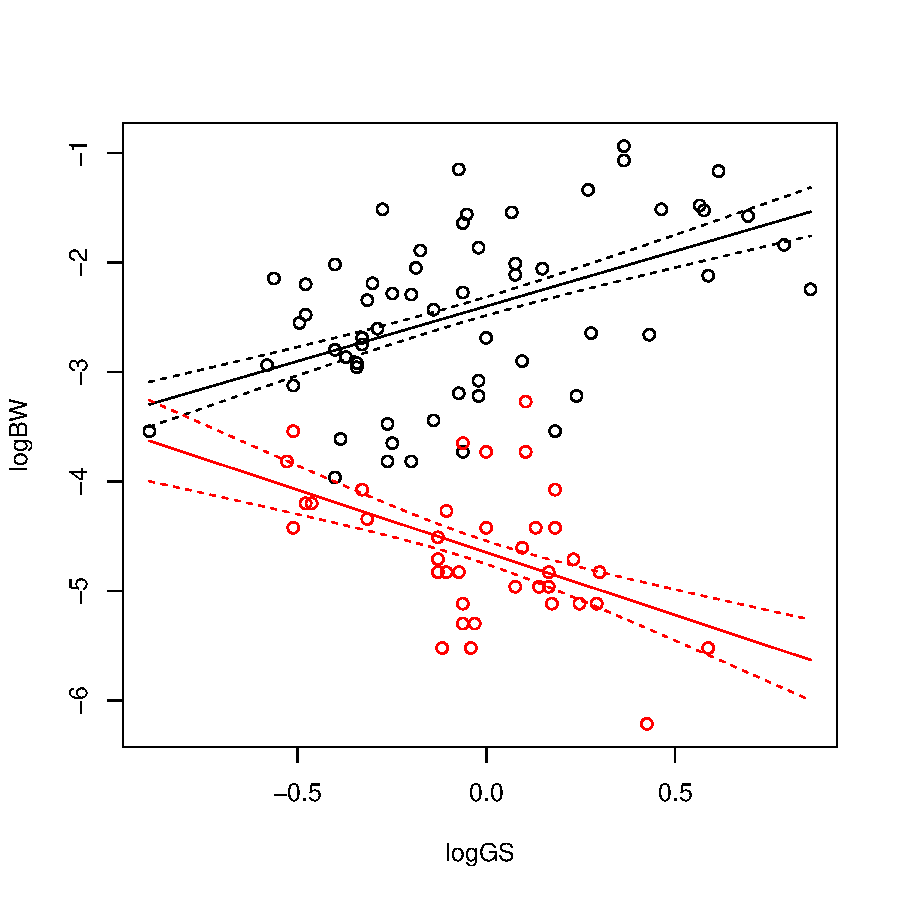
\includegraphics[width=0.7\textwidth]{odonPlot.pdf}
\end{center}  

